\chapter{Methods and Implementation}\label{cha:Method}

% längsta avsnittet i rapporten. Den består av en redogörelse av ditt arbete och den visar hur du kommer fram till dina resultat.

% Undvik egna synpunkter. Dessa framförs i Inledningskapitlet och Diskussions-kapitlet

% Ange källa till figurer i slutet. T.ex.  Source: Expedition Mondial.

% Metoddelen beskriver tillvägagångssättet – intervjuer, observationer, litteraturstudier, laborationer och så vidare. Motivera varför en viss metod valdes och vilka eventuella svårigheter som har förekommit. Metoden ska vara replikerbar, vilket innebär att en annan skribent ska kunna göra om studien med hjälp av informationen i metoddelen. Det finns en mängd böcker om olika vetenskapliga metoder. Till exempel kan en intervju utföras på en mängd olika sätt. I rapporter inom humaniora brukar metoddelen vara mer utförlig än i en teknisk rapport.

To understand the users of the app and the design possibilities, the setting and research context is described, together with a description of the collaborators and participants of the master thesis. Subsequently, study design and data collection is presented, followed by a data analysis framework that presents methods used to analyse quantitative and qualitative data. Finally, the application implementation is described.

\section{YoungDrive, Terminology and Limitations}

In this section, the organizational structure of YoungDrive and the master thesis is described, also explaining why there is an opportunity to innovate in regards to mobile technology in Uganda.

\subsection{Social Innovation and Social Entrepreneurship in Uganda} % https://www.linkedin.com/pulse/social-innovation-entrepreneurship-uganda-why-mobile-services-nissar?trk=prof-post

    This section will present background on working with mobile learning platforms, and understanding the society of entrepreneurs in Uganda.

    \subsubsection{Why Uganda is the world's most entrepreneurial country}
    According to Nissar \citep{nissar}, some facts related to entrepreneurship in Uganda are:

    \begin{itemize}
      \item Uganda is the world's most entrepreneurial country. (28\% of the population are entrepreneurs)
        \item Uganda has the second youngest population in the world (77\% of all Ugandans are below 30)
        \item Uganda has a very high unemployment rate (64 \% of people between 18–30 are unemployed)
    \end{itemize}

    % Ytterligare beskrivning av land: http://www.sun-connect-news.org/countries/uganda/

    With a high unemployment rate and little or none social security, starting a business is for many young entrepreneurs simply a tool for survival. But tough conditions can also lead to creativity, and there are as well many innovative entrepreneurs with great ideas and the aim to create positive social impact.

    As Mitchel says about entrepreneurship \citep{mitchel}, the motivation of entrepreneurship does not need to be solely wealth accumulation anymore. The activity of entrepreneurship contributes to society, in a way that is not captuted by the commercial entrepreneurship literature.

    No matter the reason of starting a business, Uganda's many entrepreneurs are contributing to the national society by boosting the economy and creating new jobs.

    \subsubsection{Why mobile services are growing rapidly in Uganda}
    One of the reasons is that the country has invested heavily in communication networks, even connecting remote rural villages with fibre optic cables and thereby connecting them to a world of information.

    As much as 65\% of the adults in Uganda owns a cell phone, which has allowed many areas in the country to skip the landline stage of development and jump right to the digital age.

    For those who hasn’t electricity at home, there are plentiful of charging booths for mobiles all over the country.

    \subsubsection{Mobile services and social innovations}
    The wide use of mobile phones has lead the way for the development of several innovative mobile services and in many cases the mobile service are way ahead of us  \citep{nissar}. In Sweden mobile banking services that allows us to transfer money through our mobile phones were made popular with Swish, introduced in 2012. In Kenya people have had similar services for the last 10 years.


\subsection{YoungDrive}

    \cite{youngdrive-web} is based on a Swedish concept, and had previously had a pilot in Botswana, when tasked with running the entrepreneurship module of A working future for Plan International. The organization fosters and educates young entrepreneurs in developing countries. They train the coaches, provide training material, and support the coaches via direction and direct support through co-project leaders and Youth Mentors.

    YoungDrive moves an entrepreneur to location, becoming country manager and "teacher". The teacher educates project leaders during four days, followed by educating coaches, which then roll out the training to the youth groups during 10 sessions, 1 session per week in average. The Community Based Trainers (CBTs) also rolls out other trainings, often simultaneously.

    For the future of YoungDrive, they want to make the CBT's even better, and collect and take use of data (monitoring and evaluation). Another motivation is scaling and monetization, as Plan International wants to increase the project to more countries, with an increased digital focus, and YoungDrive wants to be independent of project funding (i.e. a social enterprise).

    Given the above, this was a great time to introduce digital enablers for YoungDrive, where there previously had been no technology-focus, especially towards CBT's and Youth Mentors. The master thesis is the first project which focuses on digital enablers for YoungDrive.


\subsection{Roles within YoungDrive}

The \textit{country manager} trains the project leaders. It is also the main person responsible for partnerships and the quality of the YoungDrive program in the respective country. In Uganda, the country manager is Iliana Björling. She is located in the Uganda capital, Kampala, which is a strategic location because it is the same city in which the national office of the main partner, Plan International, is located. In Zambia, the country manager is Josefina Lönn, who previously was project leader in Kampala, and has held all the trainings up to this point. Now, she leads the operations and has trained the coaches in Zambia, in the new role of country manager and project leader.

The \textit{project leaders} trains the coaches and oversee the coaches, manages the coach training, and also collaborates with local stakeholders for quality assurance and to oversee daily operations.

The \textit{coaches} trains the youth. In Zambia, a coach only has responsibility for training youth in the YoungDrive program. In Uganda, this is called a \textit{Youth Mentor (YM)}, in contrast to being a \textit{Community Based Trainer (CBT)}, which also trains the youth in other programs and leads the youth saving groups. Most of the CBT's in Uganda holds sessions together with a Youth Mentor, or divides work between them, instead of being alone. The coaches are often volunteers, receiving a small scholarship from the partner organization. They are often business owners themselves. The coaches could be described as social entrepreneurs \citep{mitchel}. Many of the YoungDrive coaches (and youth) are driven by that their business can have an impact on their community, \textit{as well} as take them out of unemployment or increase their current livelihood.

The \textit{youth} are the ones receiving the training from the CBTs and the YMs, being encouraged to start their own businesses.


\subsection{Mobile Technology in Uganda's Rural Areas}\label{sec:mobile-uganda}

One of the reasons why mobile services are growing rapidly in Uganda is that the country has invested heavily in communication networks, even connecting remote rural villages with fibre optic cables and thereby connecting them to a world of information.

As much as 65\% of the adults in Uganda owns a cell phone, which has allowed many areas in the country to skip the landline stage of development and jump right to the digital age. For those who hasn’t electricity at home, there are available charging booths for mobiles all over the country.

The wide use of mobile phones in Uganda and other developing countries has lead the way for the development of several innovative mobile services and in many cases the mobile service are way ahead of us  \citep{nissar}. In Sweden mobile banking services that allows us to transfer money through our mobile phones were made popular with Swish, introduced in 2012. In the neighbouring country Kenya, people have had similar services for the last 10 years, and mobile money is since long also common in Uganda.

A prominent example of an app that has previously been developed with the target group in mind is Ledger Link \citep{ledgerlink}. This mobile banking service empowers, developed in partnership with a bank, allows saving groups in rural areas such as Tororo to save money remotely. It is developed with human-centered design methods, and has won several awards.

%For the future of YoungDrive, they want to make the CBT's even better, and collect and take use of data (monitoring and evaluation). Another motivation is scaling and monetization, as Plan International wants to increase the project to more countries, with an increased digital focus, and YoungDrive wants to be independent of project funding (i.e. a social enterprise). This was a great time to introduce digital enablers, where there previously had been no technology-focus, especially towards CBT's and Youth Mentors. The master thesis is the first project which focuses on digital enablers for YoungDrive.

%\subsection{Hybrid App Development}

The history of app and web development is rich and increasingly intertwined. First, websites were developed for desktop only, and when smartphones became popular, they were made responsive.

With today's possibilities of native mobile development or developing a native app using web technologies, there are numerous viable alternatives available if an app should function on several devices, depending on budget and preferences.

One of the main argument for developing an app in web technologies, is that the whole application, including the server, can be written in one programming language, JavaScript (full-stack).

Tools such as Apache Cordova can compile JavaScript applications into native apps. Thus, they can appear on Apple iOS and Android Play Store, as well as on the web, or installable offline on a smartphone from the computer.

JavaScript is developing rapidly as a language, as well as its ecosystem of frameworks and tools. Frameworks have emerged and matured, like Meteor.js, which makes building full-stack applications in JavaScript reliable and fast.

Previously, web hosting has been troublesome for JavaScript server applications. Today, tools such as Meteor.js and Heroku have introduced free and paid hosting for such applications, with smart bindings to code platforms such as GitHub, which makes collaboration and version handling easy.




\section{Collaborators for the Master Thesis}\label{sec:collaborators}

Collaborators in the project are the current author, supervisors, stakeholders and experts. Below, the responsibilities of these are more clearly laid out.

\subsubsection{The Current Author}
It is needed to take on several roles in the project by the current author: most notably that of a project leader, designer and developer. It is needed to balance stakeholders' different opinions and requirements, and caring for the vision in order for the project to be successful (see section \ref{aGoodDesigner} A Good Designer).

There are two groups, with the current author included in both of them, which gather at the end of each sprint for a check-up meeting. The Expert group consisted of Expedition Mondial and LiU Innovation. Expedition Mondial could help with the design process, and LiU Innovation could offer input on social innovation. The meetings mostly lasted for one hour. The Partner group consisted Iliana Björling from YoungDrive, and Lena Tibell and Konrad Schönborn from Linköping University. In Partner meetings, The Insighs from each iteration was presented and discussed. Then possible decisions were laid out, followed by discussing the alternatives. Outside of these groups, these people can also give advice in certain situations. For specific areas, there are also some experts which have been beneficial during the projects. Below, the whole team is explained: % Then I tell them about which decisions has been taken and why.

\subsubsection{Supervisors}
The supervisors are from YoungDrive and Linköping University. The YoungDrive team consists of Iliana Björling, founder of YoungDrive, and Josefina Lönn, country manager in Zambia. They are both helpful in giving knowledge on the entrepreneurship education program, and giving support. The Linköping University team consists of Lena Tibell, Professor, and Konrad Schönborn, Doctor, within the Department of Visual Learning and Communication.

\subsubsection{Stakeholders}
The stakeholders are considered YoungDrive and Plan International. \textbf{YoungDrive} is the client of the work, and their needs should be satisfied. This person is mainly represented by Iliana Björling, who is part of the YoungDrive Strategic Management Team. Using service design, the project leaders in Uganda and Zambia, are also considered stakeholders: Josefina Lönn in Zambia, and the two co-project leaders in Uganda. Finally, the most important stakeholder of all according to service design, is the actual users: the coaches. They should be the main consideration of the work.

\textbf{Plan International} is the organization allowing for all the interactions with the end users in Uganda. A similar organization is operational in Zambia. They are the ones that are providing facilities, organizes transport, etcetera. They in turn, have the organization Community Vision, which organizes the coaches. If Plan International or Community Vision does not appreciate of the project and the collaboration, then the interactions with the coaches will not be possible.

%\textbf{Linköping University} is a stakeholder, as the supervisor (Lena Tibell) and examinator (Camilla Forsell) determine if the work is a valid master thesis or not. Also, LiU Innovation is interested in supporting continued work with the project, and their representative Peter Gahnström gives advice on social innovation and how this project can continue in the future during expert meetings.

\subsubsection{Advisors}
Since the development country context is new to the current author, there are also specific experts advised in the project. For design process, Susanna Nissar and Erik Widmark from Expedition Mondial has supported with all of their knowledge within service design. Julien Tantege, Research Specialist at Grameen Foundation, has been kind to offer support before and during the work, sharing their insights from related work, and giving feedback during ideation. She has experience doing technical development for rural areas. For pedagogical development, Henrik Marklund from edtech startup Knownly in Sweden has given support with regards to building skills within digital learning. For feedback for how the work relates to social innovation, Peter Gahnström at LiU Innovation has offered feedback.


\section{Describing the YoungDrive Coaches and the Research Context}

The biggest challenge with regards to time constraints and cultural differences is that it is difficult to understand the target group of the app. Therefore, the whole design and development process will take place in Uganda, with several interactions with the intended users. The work was carried out from Hive Colab, a co-working space and an innovation hub. The work is done mainly from Kampala, because that is where YoungDrive is situated, meaning that there is still a long distance to the coaches and youth in Tororo, which is located near the Kenyan border. Another challenge with being in Uganda compared to Sweden is that internet speed and access is worse, especially outside Kampala.

 The interactions took place in either Uganda or Zambia, in the locations where training of the coaches and youth takes place.  There were a number of resources made available to support the work, for example the YoungDrive manuals. Each youth is given a \textit{Participant manual}, describing each week of the 10-week YoungDrive program. Coaches are also given a \textit{Coach guide}, which describes how to carry out and teach each week's topic during the youth training. As most of the coaches did not have smartphones or tablets, four smartphones (3 Android, 1 iOS) and ten tablets (3 Android, 7 iOS) were brought from Sweden. All of these devices had a web browser and access to an app store. These were either donated, borrowed or bought devices. During the user tests, also using a laptop would be tested. The following section describes the Ugandian and Zambian coaches and their businesses.

\subsection{Social Characteristics and Businesses in Uganda}

According to statistics gathered by YoungDrive during 2015 evaluations \citep{youngdrive-statistics}, there are a number of considerations to make regarding the coaches in Uganda. This regards entrepreneurship experience, technical access, and language, see a summary in figure \ref{fig:ydStatistics}. Taken together the coaches' and project leaders' technical skills are currently low, and this needs to be in consideration when designing the app. Regarding language, English can be used in the coach app.

\begin{figure}[h]
    \centering
    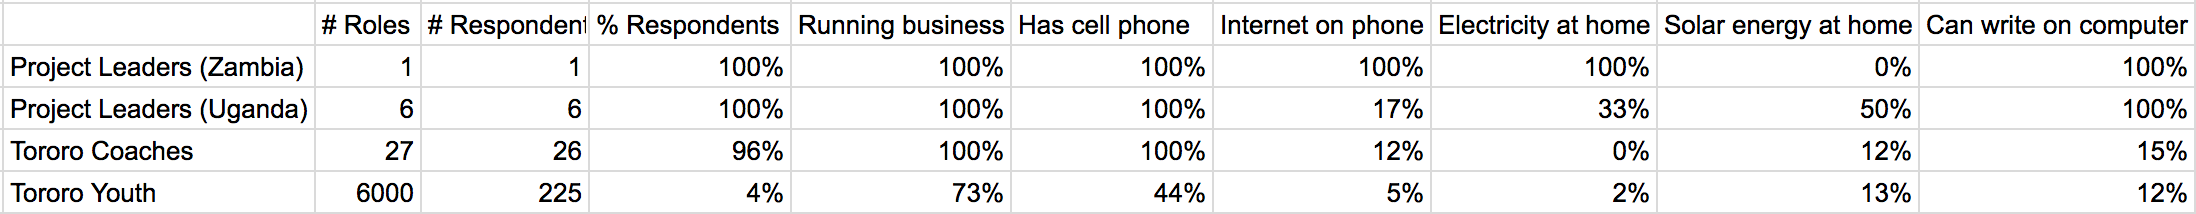
\includegraphics[width=1.0\textwidth]{ydStatistics.png}
    \caption{Table showing entrepreneurship experience, technical access, and language between Tororo coaches and the project leaders in Uganda and Zambia. All of the Tororo coaches run a business (with a majority running more than one). This means they do have practical experience of running a business outside of the YoungDrive coach training. While all have a cell phone, smartphones are very uncommon - only 3 uses Internet on the phone, every day or weekly (mostly for Facebook or email). Regarding power, none has power at home, 3/26 has solar, and only 4/26 can write on a computer. While about half of the asked Uganda youth can not understand (129/225), read (133/225) or write (132/225) English, most of the coaches in Uganda are proficient. These characteristics are similar for youth and project leaders as well.}.
    \label{fig:ydStatistics}
\end{figure}

The coaches in Tororo are divided into three different regions. Based on region, income and experience, they run different kinds of businesses. \footnote{In Uganda and Zambia, a small-scale business is typically not registered. Thus, the coaches' definition of a business can be more generous.} In Tororo, the coaches' businesses range from: pineapple, water melon, onion, chili, bakery, catering, corn, beans, fabric, plastic products, bird farm, milk, fish, ground nuts, cabbage, tomato, hairdresser, sewer, shop and rice. For photograph of the environment, see figure \ref{fig:tororo}.

\begin{figure}[h]
    \centering
    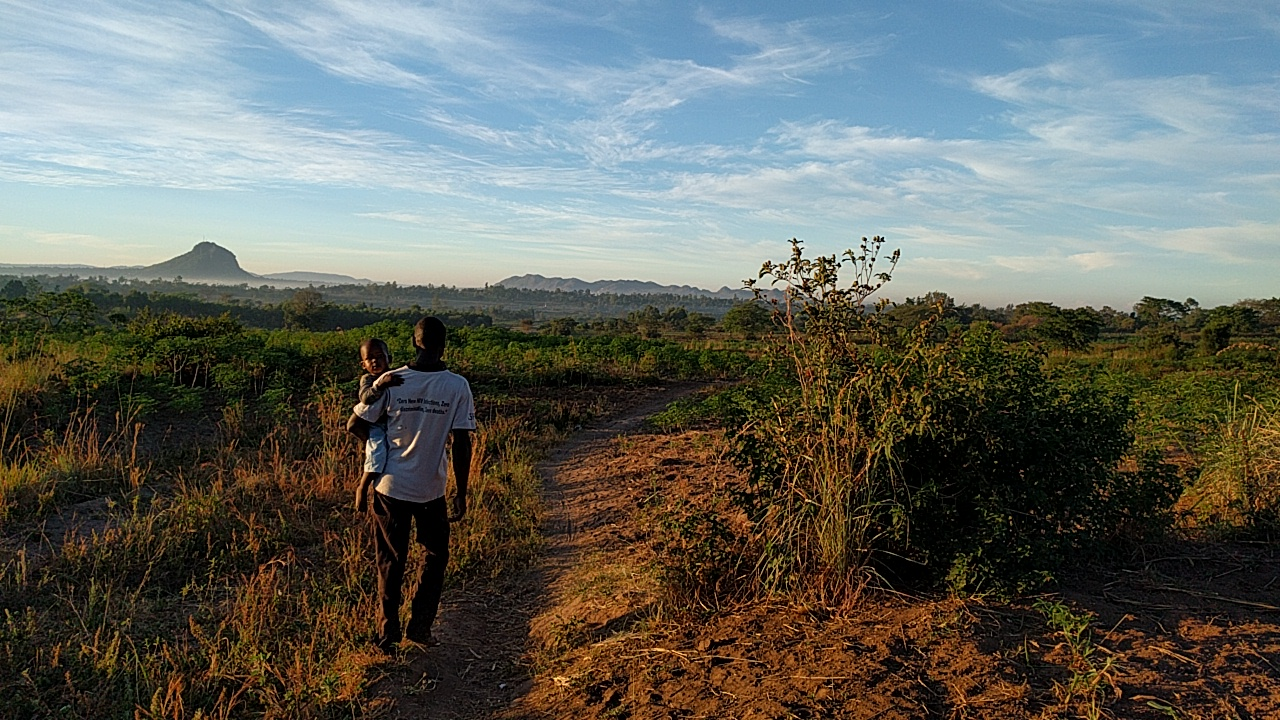
\includegraphics[width=0.7\textwidth]{stayover.jpg}
    \caption{One of the co-project leaders showing the rural part of Tororo, where crops are growing close to where he lives.}.
    \label{fig:tororo}
\end{figure}

In Tororo, there are 2 Project Leaders. one project leader's business range from: bakery, corn, pig farm and plastic products. The other person's business range from: silver fish, beans, corn, and bird farm. In comparison, in Kamuli, there are 4 Project Leaders. Their businesses range from: selling office supply, motorcycle taxi, bird farm, pig farm, green pepper, corn, cabbage, tomato, aubergine, chipati ("bread"), chilli, and charging of cellphones.

Among the youth, the top 8 most popular businesses in Tororo, with 134 respondents, are corn, cassava ("potato"), saloon, fish, making of bricks, beans, brooms and rope. These range from 9 for corn (6.7\%) to 5 for rope (3.7\%).

\subsection{Social Characteristics and Businesses in Zambia}
During the visit in Zambia, the coaches had not yet formed their youth groups, and started their own teaching. Regarding characteristics, ages ranged from 21-39 years old (26.8 average). Other data available about the coaches were notes of the Zambian coach job interviews, which could be compared with during quiz analysis \citep{yd-zambia-interviews}. Compared with Uganda, 9 out of 10 had business experience.

%3 were mentioned as being shy during the interviews. They lived from 10-90 minutes outside of town (33 minutes average).

%Regarding motivations for being a coach, 50\% had an emphasis on benefiting the community, and 90\% had personal reasons.



%Care for oneself:
%\begin{itemize}
%\item Learn business %(7)
%\item More skills %(2)
%\item Get idea
%\item Expand business
%\item Benefit CV
%\end{itemize}
%
%Care for community:
%\begin{itemize}
%\item Empower %(2)
%\item Teach business
%\item Leadership
%\item Share
%\item Stop bad behaviours of youth
%\end{itemize}

%regarding experience, 8 had trained youth before, 8 had been a leader before, 9 had business experience. Regarding YoungDrive, they said they could handle training between 8-30 youth (19.8 on average) per group. They could have 1-5 groups per coach (average 3.0), totalling a range between 8-101.5 youth (average 59.8).


\section{Study Design and Data Collection}

  As a computer expert with social skills needing to design and develop an app for a unfamiliar cultural and socio-economic context, it was needed to quickly become a good designer.

  The technical aspect of the project was but one. It was needed to learn how to develop hybrid apps in JavaScript that worked offline, and had an online back-end. However, those are merely the technical demands.

  It was needed to quickly become a good designer, not mainly from a perspective of graphic design or interaction design, but \textit{how} to explore, design, and implements what the user needs from the requirements "fun, user friendly, and good for learning". The approach used to learn design from these perspective was to read extensive literature, consult a diverse set of experts, and be humble and curious in interactions with the end-users and stakeholders.

  In the following section, the creation and implementation for a suitable design process is described, together with the study design and data analysis for each iteration of the project.

%Har gått igenom planeringsrapporten lite noggrannare idag och ser två saker som vi kanske ska borde fånga upp under arbetets gång.

% Under 2 Purpose står det ett upplevelsemål från Young Drive. Bör vi mäta detta upplevelsemål om det stämmer med deltagarnas faktiska upplevelse, d v s ska vi försöka få in det under 3 Research Questions?

% På våra avstämningsmöten borde vi också följa upp dina Research Questions så att kundinteraktionerna och servicedesignmetoden tyligt leder dig framåt mot dessa mål.
%* Reflektioner på vilka designprinciper som bör väljas? (utifrån kundinteraktioner)
%* Reflektioner angående tekniska begränsningar?
%* Reflektioner på processen?

\subsubsection{Creation of Design Process}
As there was a unfamiliar target group - mostly young Ugandians with little or no experience of smartphones - service design thinking would benefit true understanding of cultural context and in-depth empathy for the end users.

Tools and methodology in service design were chosen with the help of Expedition Mondial in Stockholm, who provided education and coaching.

At the same time, the end result would be a digital artefact (an app), which is not common in service design.

While this product could be though of as a service, the tools and methodology would benefit to borrow from Agile methodology and Interaction design.

I'm the computer expert kind of designer \cite{lowgren}, adjusted to agile methodology and interaction design, but aspiring to be a socio-technical expert. Expedition Mondial are experienced with service design, aspiring to be more of computer experts.

This led to the joined development of a Digital Service Design method, co-created by the both.

%Expedition Mondial helped with a method for creating a MVP of the digital support for the coaches, so that the app was developed from the perspective of the end users and the education and a "learning by doing" mentality.

%The suggested design process was designed with them after a start-up meeting on Skype, and an education day in Stockholm. During that day a crash course in service design was given, then creating a common plan for the future work based on my needs (see Appendix: Original Time Plan \todo{Add reference}). They also recommended service design literature. These were the methods chosen in each iteration.

The result is that the design and development phase in Uganda is an iterative process with the human in focus. The process is built on top of service design process and methodology, while in-line with digital design practices.

\subsubsection{Implementation of Design Process}
There were four iterations. The first iteration follows Service Design, not starting the app development, while the other three follows the new methodology, Digital Service Design.

In iteration 1, there is a very broad scope, without digital focus, where iteration 2, 3 and 4 introduces and narrows down the project into a digital solution.

Expedition Mondial gave support in each iteration, helping with refinements of each iteration as learnings happened along the way, and they were able to educate me during the different stages with methodologies whenever necessary.


\subsection{Implementation of Methods for Data Collection and Data Analysis}

This section describes the implementation of methods for each iteration's interactions, in regards to collecting and analysing qualitative and quantitative data. Figure \ref{fig:methods} is made to assist the reader in the iterations' different focuses.

%study design, application development, and for data analysis theory.

\begin{figure}[h]
    \centering
    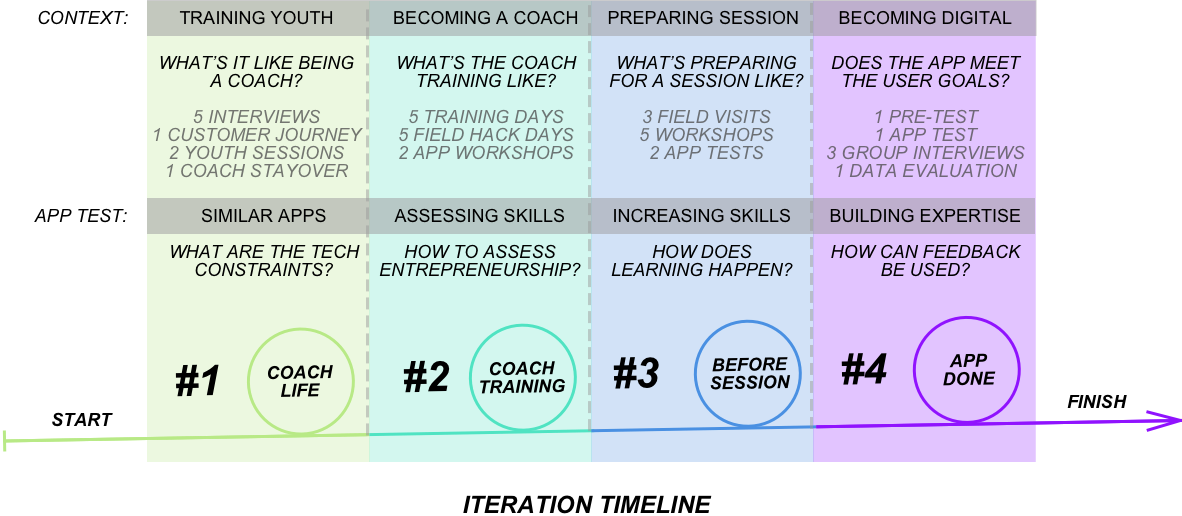
\includegraphics[width=1.0\textwidth]{iterativeprocess2.png}
    \caption{Each of the four iterations had a unique context, app test focus, and research focus. The loops is meant to remind that an iteration consists of three steps before Interactions with the coaches: Insights, Ideation and Trigger material. For more information, see section \ref{digital-service-design} Digital Service Design.}
    \label{fig:methods}
\end{figure}

%Methods w/ Analysis
%----
%
%5 Interviews - Notes - Questionnaire for Customer Journey
%1 Customer Journey - Clustering - Personas
%2 Youth Sessions - Shadowing - Needs
%1 Coach Stayover - Empathy - Design Ethnography
%
%5 Training Days - Observations - Understanding entrepreneurship training
%5 Hackathon Days - Interviews - Notes and Sketches
%2 App Workshops - Co-Creation/Co-Refinement - Sketches and Needs
%
%3 Field
%
%Acitivity
%App test observations (group)
%
%App test observation (individual)
%- Affective reactions (5 Why's, think aloud)
%
%Analysis: Interaction design evaluation (desirability, usability, utility, %pleasurability)
%
%Customer Journey Map
%- Activities
%- Behaviour
%
%Written responses (individual)
%- Right/wrong
%- Time
%- Number of tries
%
%Interviews
%- New insights
%
%Data Collection w/ Analysis
%----
%
%Customer Journey Map w/ clustering
%
%Pre-study w/ Quantative analysis
%
%Written quiz responses w/ Quantative analysis
%
%Digital quiz responses / Quantative analysis + Statistical analysis + %Parallell coordinates
%
%Quiz questions 1 w/ Bloom analysis
%Quiz questions 2 w/ Bloom analysis

%\input{implementation/iteration-1}

%\input{implementation/iteration-2}

%\input{implementation/iteration-3}

%\input{implementation/iteration-4}


\subsection{Iteration 1: Uganda Coach Visit}

% How was this iteration designed?

Following the service design sequencing, the first iteration had a very broad scope and truly is a service design iteration: "From your perspective, what is it like being a coach?". \footnote{A coach meaning either a Community Based Trainer (carrying out all the trainings), or a YoungDrive coach, depending on who was asked the question.} \cite{lowgren} was used how to start the project, meaning that the purpose was to get a preliminary understanding of all important aspects, and build relationships with all stakeholders.

%The project started with a startup meeting with Shifteh from Plan International in Kampala, together with Iliana. From there, I did research and met with Grameen Foundation and Designers Without Borders, before going to Tororo to research "What's it like being a YoungDrive coach?", and determining how advanced an app could be to solve challenges that the coaches face.

Insights depended heavily on interviews with all the stakeholders  (2 with Plan International, 3 with YoungDrive), and local experts (1 visit each at Grameen Foundation and Designers without Borders, 1 workshop with Mango Tree), since no Interactions with users had been made yet. Also, knowledge and connections were made with the Kampala tech scene as much as possible, from the new home and office in Kampala, working at the tech hub and co-working space Hive Colab.

Ideation were about creating a questionnaire guide for the interviews, a co-creation workshop using "Customer Journey Map", and identifying how the app test should be designed to test their existing knowledge (and be informed of the design preferences of the YoungDrive app).

Trigger material was the finished questionnaire guide (constructed with Expedition Mondial) a written plan for the co-creation workshop ("A day as a coach"), and a written plan for testing the quiz app Quizoid and the language learning app Duolingo, and a schedule for the interactions.

The interactions were focused on design ethnology, getting to know and learn from people in a different culture, namely the coaches. The focus was on the their needs, motivations, and context.

To accomplish these, four days were spent in Tororo, with one day of travel. There were four face-to-face-interviews,
one meeting with Plan, one meeting with the local partners, two workshops, one coach stay-over, and two youth session visits (one of the youth sessions are observable via figure \ref{fig:youthsession}.

\begin{figure}[h]
    \centering
    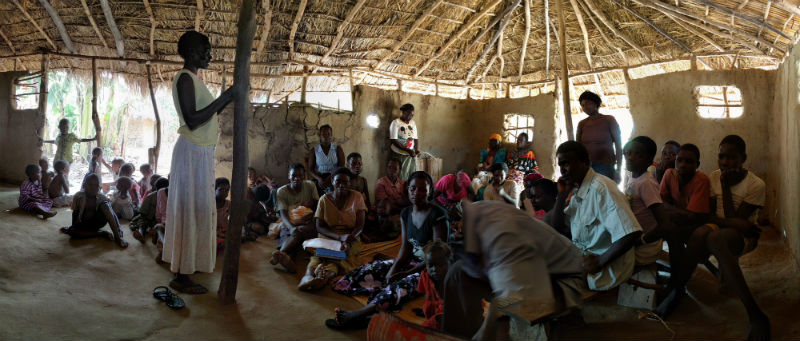
\includegraphics[width=0.7\textwidth]{youthsessionSmall.jpg}
    \caption{Photo from the location where one of the youth sessions were held. Here, a CBT in Tororo teaches youth in basic sales and marketing.}
    \label{fig:youthsession}
\end{figure}


\subsection{Iteration 2}

This time, the iteration has a more detailed scope, with a hypothesis on what needs the app should meet in the end, and create lo-fi and hi-fi trigger material to meet those needs.

A co-creation workshop started the interactions, followed by repeated app tests at minimum one session per day, always followed by a feedback round, so the app and the tomorrow's question set creation could be improved for the next day. At the end of the week, there was a co-refinement workshop of the current hi-fi material, and also lo-fi material for the new version of the app.

\subsubsection*{Creation of questions}
Project leader Josefina in Zambia refined Iliana's first question sets, prepared for my visit in Zambia. Josefina created question sets with Bloom at the back of her head, also taking into account the structure and the order of the coach manuals, what it means being a coach within the topic, and lastly scenarios.

\subsubsection{Trigger material used}
A hi-fi trigger material was done, a very basic quiz app, keeping it as simple as possible (see Application Implementation, Iteration 2). All of the devices (tablets and smartphones) that I had available were brought to Zambia.

I added Josefina's questions to the app, and installed the app to all of the devices. This process was repeated for all the days, Sunday-Friday.

\subsubsection{Design workshop \#1 in Zambia}
The coach training started with me having a design workshop with the coaches, not showing them the app that I had created. The co-creation workshop was made to identify important functionality in the minds of the coaches.

\begin{enumerate}
\item Since the knowledge about smartphones and apps were low, I started by introducing these topics.
\item All were familiar with Facebook, so thus I showed the Facebook app. Me wanting to know what the app would look like if the coaches would have designed the app, I first needed to train them how to design an app via drawing wireframes.
\item Using postits, they started with during limited time drawing the start view from the Facebook app.
\item Then, they were asked to draw what they thought happened on the friend icon click, drawing the view on another postit.
\item Then, the mission of the YoungDrive app was described. They were then divided into two teams, having limited time to draw the best imaginable YoungDrive coach quiz app they could. First, they designed the app from the top of their heads. They then pitched their results to each other.
\item On the next iteration, they were to suggest and design improvements how the app should be designed to improve learning, not only assessment. They then again pitched their results to each other.
\end{enumerate}

\subsubsection{Assessment via quiz}
At the end of each day, the app was used to test the coaches' knowledge. Each coach got either a smartphone, tablet or computer. The coach first took the quiz for the most recent session, and could then choose what to do next.

As there were no back-end developed, Josefina by hand documented the scores of each coach, writing the name of the coach, the session, number of correct answers, and what questions had been answered wrong.

Josefina then, when planning the next day, looked at the statistics, looking for trends that would inform the sessions for the following day.

She also evaluated the quality of the questions, before creating the new question sets for the next day.

\subsubsection{Experimenting with quiz before or after the session}
Since the coaches appreciated the app so much, we felt tempted to try what would happen with fun and learning if we tried using the app \textit{before} a session instead of only after. During the rest of the week, we continued, finally finding preferences and tendencies from the coaches, via observation, interviews, and survey.

\subsubsection{Experimenting with design of questions}
During the week, extra tests were done to test the following:

\begin{itemize}
\item Number of questions per quiz
\item Single-answer questions or multiple-answer questions
\item Framing of questions
\item Challenge level of questions
\item Determining what made a question hard
\end{itemize}

\subsubsection{Interviews with Josefina}
At the end of each day, an evaluation interview was held with Josefina. At the end of the week, a final interview was held.

At the end of Day 5, Josefina and I discussed what it would look like to not record the answers manually, but pushing the results online. A co-creation workshop was held, where she drew an Educator Dashboard.


\subsection{Iteration 3}

Because of the many research and functionality needs, the study design of Iteration 3 became very important. A lot of development and ideation needed to be done.

\subsubsection{Iteration 3: Purpose}
Iteration 3 had an even more detailed scope. Since the app now succeeds with the first use case, the coach training, now the focus could be on "learning at distance".

\subsubsection{Pedagogical model}
It was chosen that "Are you sure?" + Improve would be included in the hi-fi material, a flip-card approach would be tested as a lo-fi material, and to "record answer via voice" could only be presented as an idea during a field interview (experts said there would be usability issues, and the 1st-time smartphone user agreed). The Gold/Silver/Bronze method was included into the hi-fi material.

\subsubsection{Test on a Kampala entrepreneurship student}
Also, instead of only testing the app in Tororo, a test was held in Kampala, to get feedback from an entrepreneurship student.

\subsubsection{Test in Tororo}
As Plan International staff are not allowed to support visiting coaches in the field during local elections, the co-project leaders in Tororo were consulted to carry out the field trips, so that it was still possible to attend the youth group meetings.

For the interactions, a big app test was held, a group interview was held, and then they were divided into co-creation workshop groups, with a presentation in the end.

%Before the workshop, the wished functionality and goals were well formulated. It was also discussed beforehand how to best design the workshop, together with Linköping University and Expedition Mondial.

There was another partner meeting, with Plan International and Community Vision present. There was an app test with all of the coaches, "Testing the YoungDrive coach app", followed up by splitting into six workshop groups based on solving different problems discovered during the test.

The following day, there were three field visits to CBTs, observing how they prepared themselves for a youth session, and then testing the app for assessing and becoming prepared for a session.

After the app tests, it was tested with a lo-fi prototype that the coach thinks aloud about the question, \textit{before} receiving the multiple-choice answers. This approach proved to be great for learning, and could be a great addition to the hi-fi material. Interestingly, this test was done as a live quiz, and if the interviewee could not answer the question directly, the audience were asked and tested if they knew the answer (raised hands), and if nobody knew the answer, it was tested which of the multiple-choice alternatives they found most likely.

During the afternoon, we divided into 5 groups focusing on improving the app experience for the coaches.

On Wednesday, the coaches from the field visits were gathered for a workshop. The purpose was to see how they acted when given the challenge: "Get 100\% correct answers in one go, on the hardest quiz". A co-creation workshop ("Educator Dashboard") was held in parallel, with 3 CBTs and 1 project leader respectively.


\subsection{Iteration 4: Uganda Summative Test}

The focus of iteration 4 was a summative test. First, a pre-test was carried out in paper, including questions about the coach and an entrepreneurship quiz, based on a well-known study \citep{general-entrepreneurship-quiz}, see Appendix \ref{cha:pre-test}. During the test, this was the first time that the app could send data to the server. Data was sent whenever a quiz was started, and whenever a quiz was finished. The group was divided into two, the ones who brought manuals and they who did not. Those that had brought manuals, could use these with the app, see figure \ref{fig:appevaluation}.

\begin{figure}[h]
    \centering
    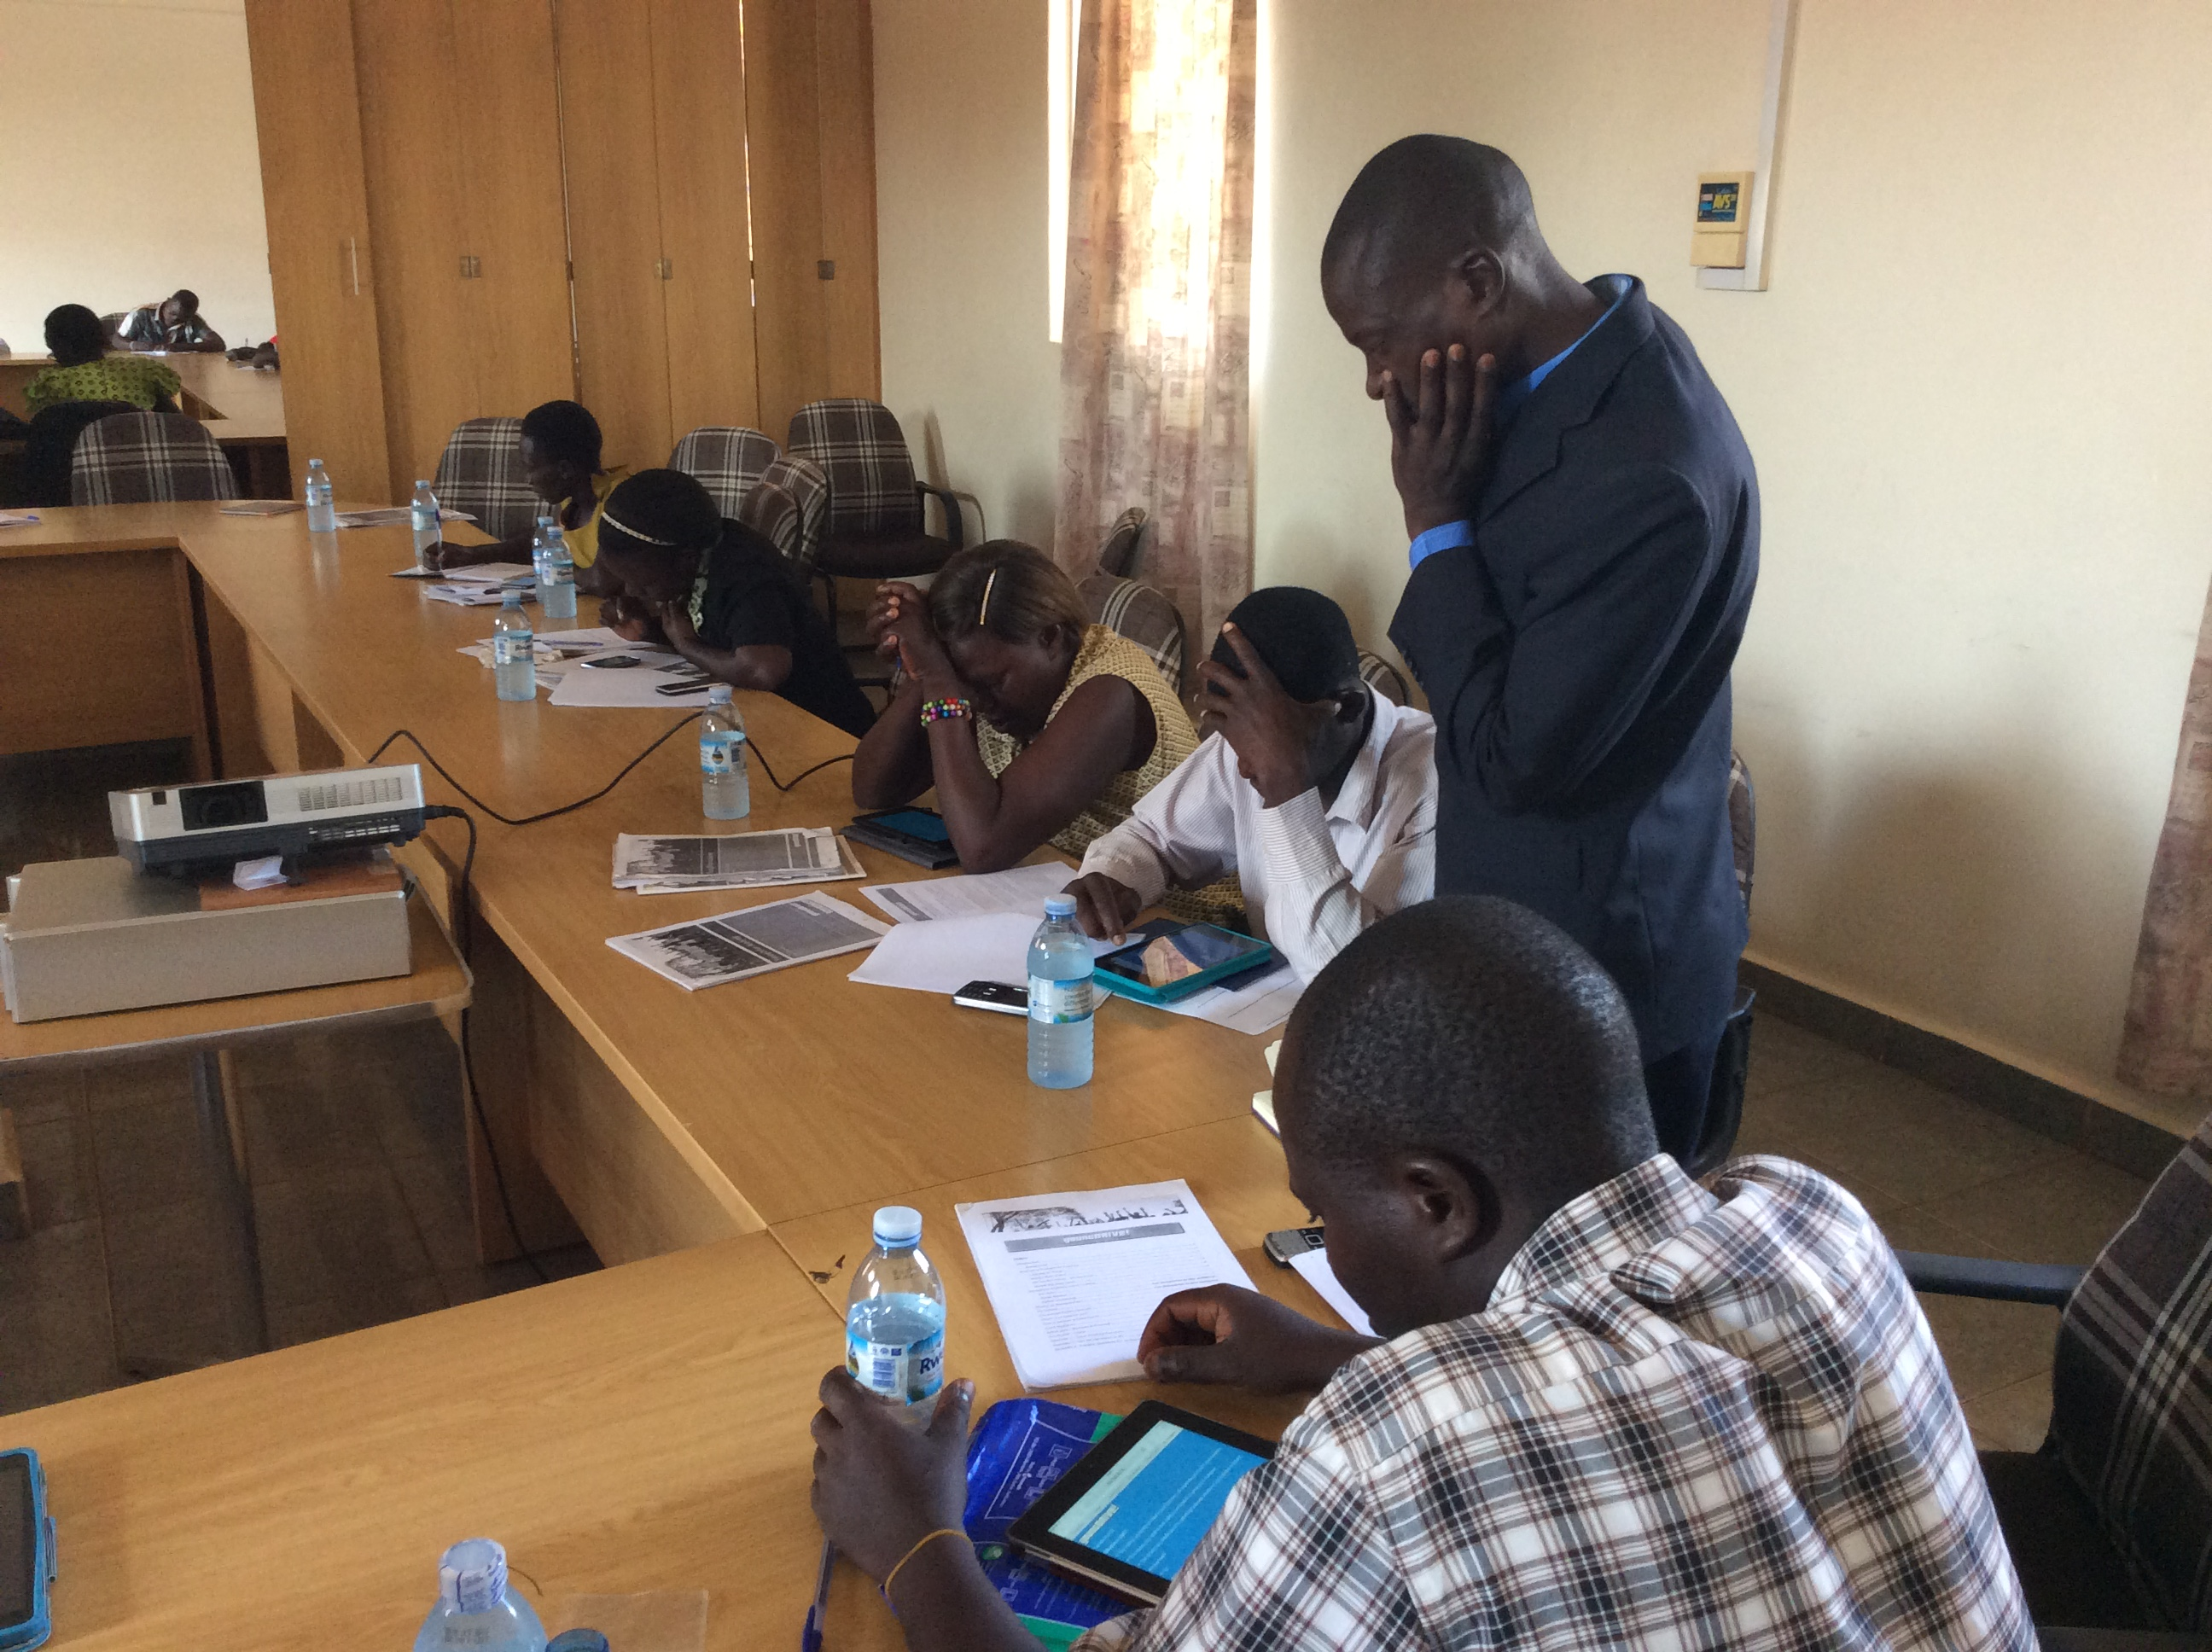
\includegraphics[width=0.7\textwidth]{appevaluation.jpg}
    \caption{Coaches answering the app questions for topic quiz 3 on Financial Literacy, and the coach guide quiz 9 on Action Plan.}
    \label{fig:appevaluation}
\end{figure}

After the test, every coach was divided into one or three groups, on random. In these groups, they were asked:

\begin{enumerate}
\item Why do you think you were correct or incorrect?
\item Do they like the app?
\item Are you stimulated by the app?
\item What did you like?
\item What did you not like?
\item When do you want to use the app?
\item When are you not able to use the app?
\end{enumerate}

To analyse the paper-submitted data, all of this was combined first into a Google Spreadsheet (the app results were also recorded in paper, but only as a backup). Data collection was done by the app itself, which pushes data to server whenever online (it saves quiz start, and quiz finish).

%The next day, a small app evaluation and co-creation workshop was held for the Educator Dashboard, and the final version of the app. Also, a test was done with the Plan Tororo staff.

%Back in Kampala, a presentation was held with Plan International. Back in Sweden, a presentation was held with the YoungDrive Strategic Management Team.



\section{Data Analysis Theory}

%\todo{Lägg till overall data table}

%Methods to choose from for analysing (i.e. what I did during the interactions, to test and analyze my app)

%Partly data collection done via app, but also all the observations

The results from each iteration needed to be analysed, using the methods outlined in section \ref{sec:data-analysis}. Depending on the kind of activity and results gathered, different data is collected.

For qualitative methods, the output is almost always observation notes, which are then concluded into insights. These insights, can then sometimes be used in the below analysis methods.

For quantitative data, the output is almost always quiz results or data about the coaches. Before analysis, how this data has been processed is clearly described in chapter \ref{sec:data-analysis}.

Below, an overview of which data analysis method was used for what data is presented. The tools and iteration the tool was used in, is outlined below as a summary:

Qualitative data analysis:
\begin{enumerate}
\item Need groups and Personas (\#1)
\item Customer Journey Map (\#1)
\item Sprint backlog (\#1, \#2, \#3, \#4)
\item Sprint demo (\#1, \#2, \#3, \#4)
\end{enumerate}

Quantitative data analysis:
\begin{enumerate}
\item Correlation in Google Sheets (\#2, \#3, \#4)
\item Correlation in R (\#4)
\item Logistical regression in R (\#4)
\item Parallel coordinates visualisation (\#4)
\end{enumerate}

\subsection{Iteration 1: Uganda Coach Visit}

In iteration 1, the following activities were carried out and then analysed:

\begin{itemize}
\item Stakeholder interview (for Need groups)
\item Coach interview and field visit (for Need groups)
\item Workshop (for Customer Journey Map)
\item Smartphone test (for Need groups)
\end{itemize}

\subsection{Iteration 2: Zambia Coach Training}

In iteration 2, the following activities were carried out and then analysed:

\begin{itemize}
\item App test observations (for Sprint backlog)
\item Quiz results (for Sprint demo)
\item App design workshop: use case 1 (for Sprint backlog)
\item App design workshop: use case 2 (for Need groups)
\end{itemize}

\subsection{Iteration 3: Uganda Formative Test}

In iteration 3, the following activities were carried out and then analysed:

\begin{itemize}
\item App test observations (for Sprint backlog)
\item Service Mini-Sprint - 5 workshops (for Sprint backlog)
\item Field visits (for Sprint demo)
\item Small formative app test (for Sprint backlog)
\item Big formative app test (for Sprint demo)
\end{itemize}

\subsection{Iteration 4: Uganda Summative Test}

In iteration 4, the following activities were carried out and then analysed:

\begin{itemize}
\item Big summative app test (for Sprint demo and quantitative analysis)
\end{itemize}

Data analysis of quiz results were done first by a general overview in Google Sheets, by statistical analysis in R, and by a parallel coordinates visualization. The process to do this, is described below.

\subsection{Analysis Implementation of Quiz Results and Pre-Data}

In this section, the steps needed to analyse the quantitative data is explained in detail, so that others can use a similar approach. In this example, quiz results are from iteration 4, but a similar approach has been taken with the manually recorded quiz results from iteration 2-3 as well.

Data analysis of quiz results was done first by a general overview in Google Sheets, by statistical analysis in R, and by a parallel coordinates visualization. The process to do this is described below.

\subsubsection{Step 1: Data Acquisition from Server}

It was desired to store the data in Google Sheets, thus it was necessary to collect the MongoDB database content, and convert JSON format into a Google Sheets-readable format, like CSV. Multiple approaches were tried, and the Google Chrome extension called Magic Json \citep{agaze} was the one that worked without problems.

\subsubsection{Step 2: Data Acquisition from Pre-Study}

The Pre-study data acquisition was done by instead of looking at the paper-submitted pre-study evaluation forms, using the data processed into Google Sheets.

\subsubsection{Step 3: Data Enhancement of Server Results}

This section presents how data from the server was processed, to enable visualization mapping. To make the data easier to work with, the columns were reordered, and made sortable and filterable. Some columns were given conditional formatting, so it would be easier to spot irregularities, see figure \ref{fig:resultsColored}. After this, some observations could be made.

\begin{figure}[h]
    \centering
    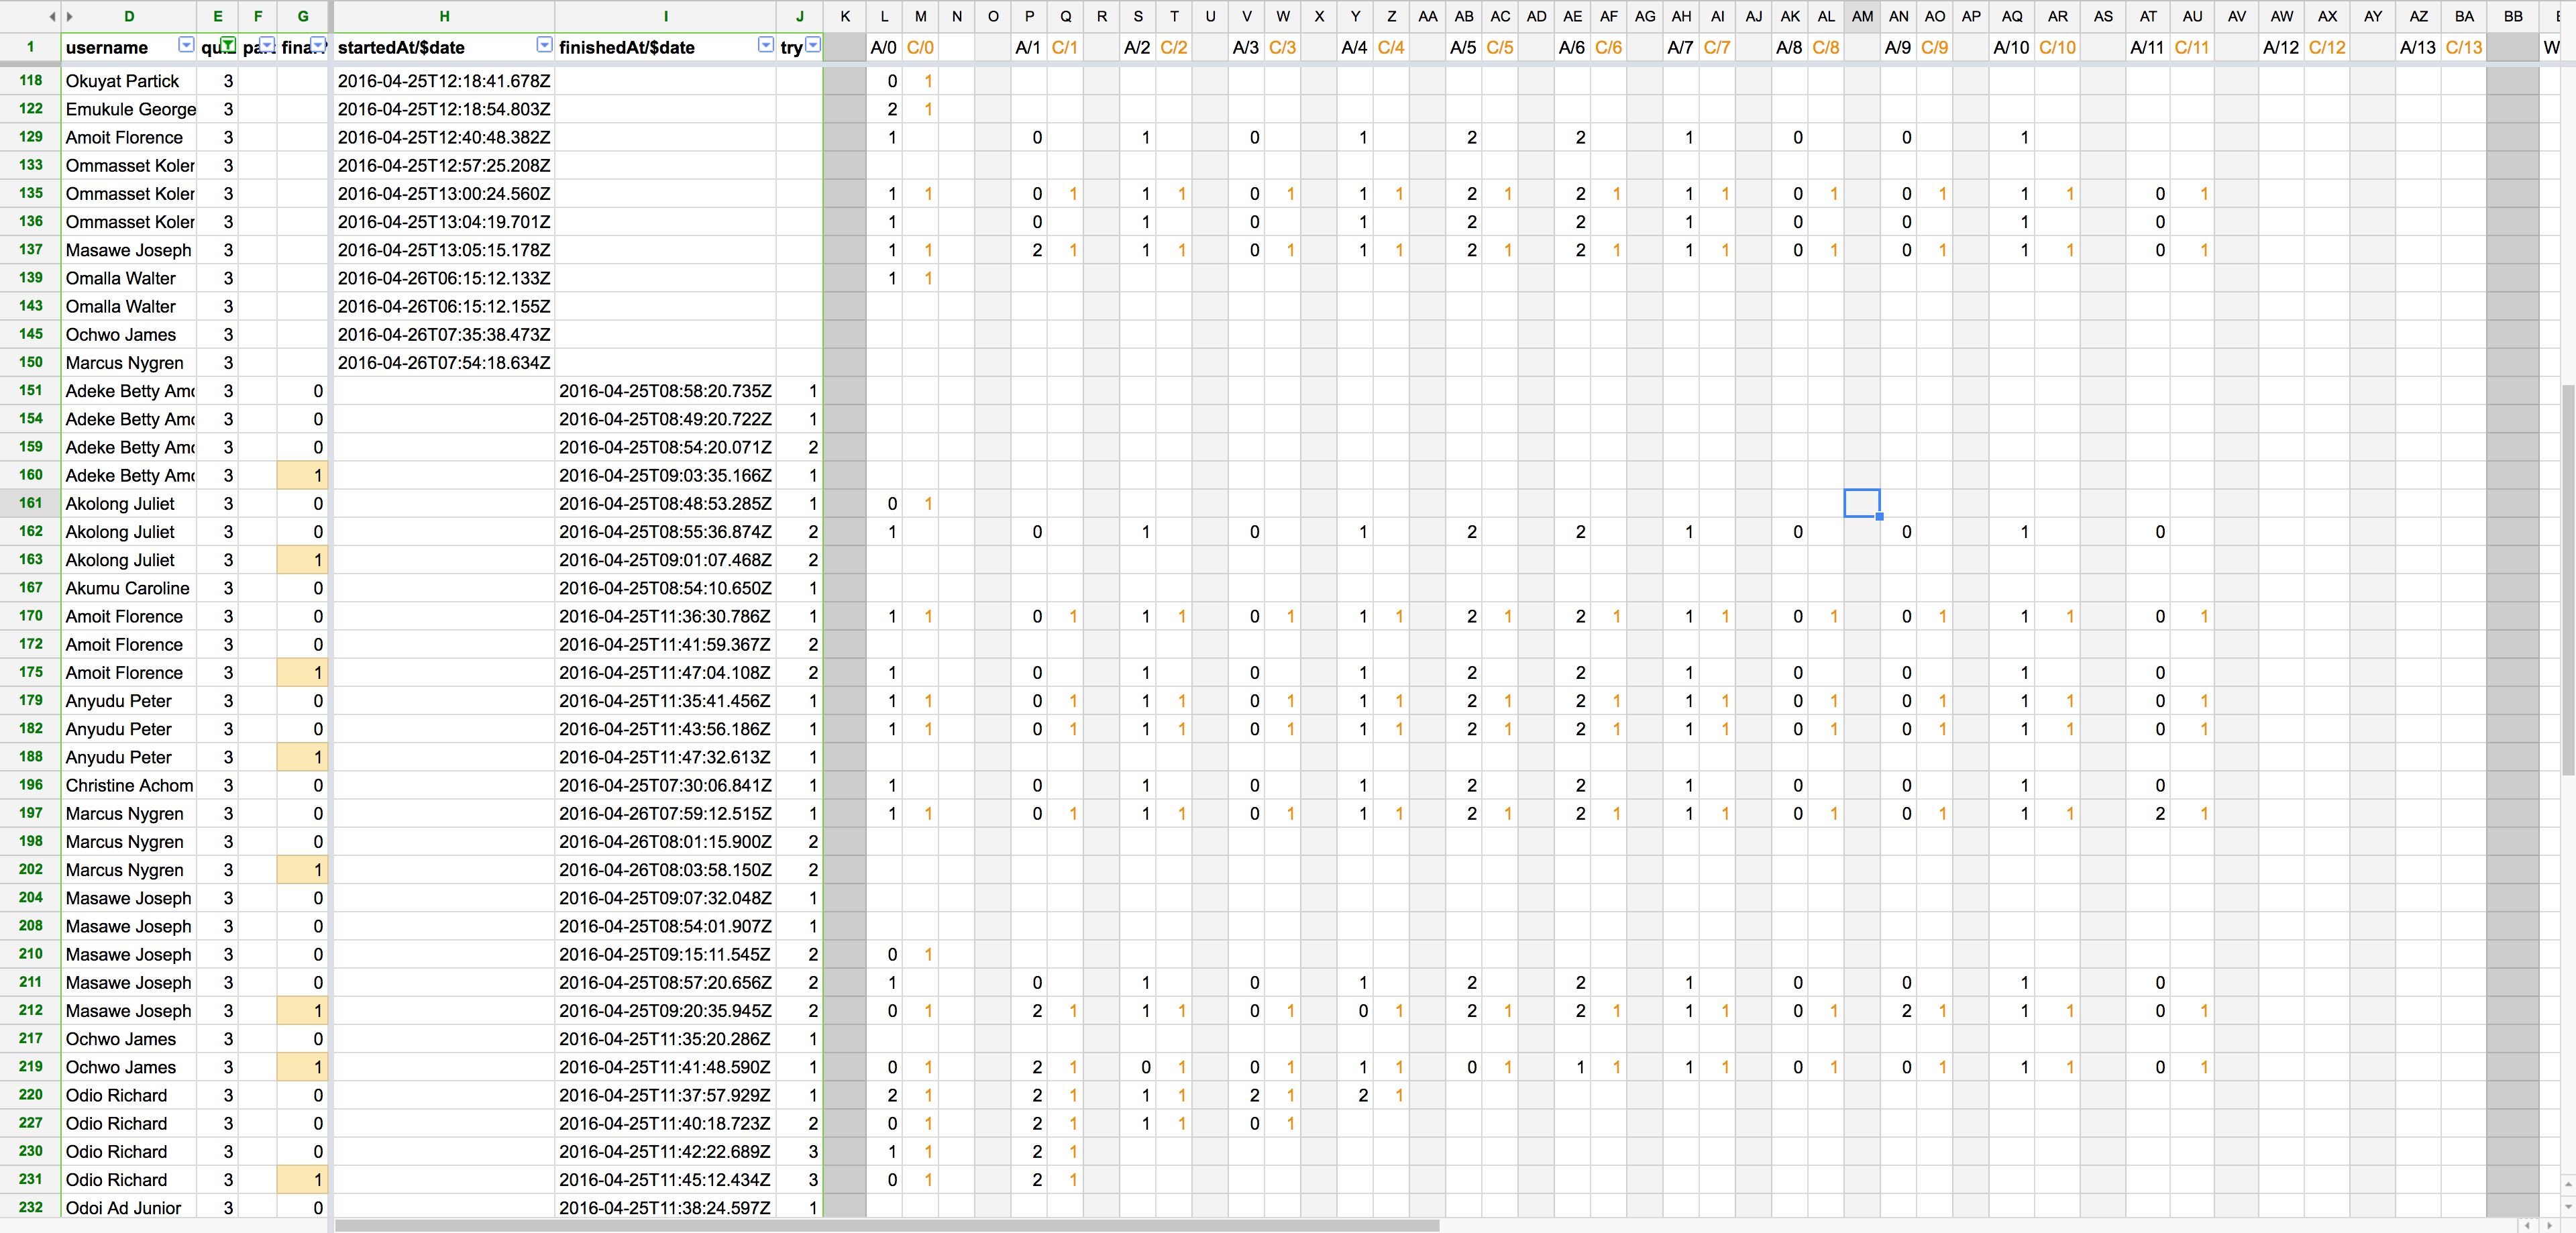
\includegraphics[width=0.9\textwidth]{analysis/resultsColored.png}
    \caption{The quiz results collected in a Google Sheet after data enhancement. In this figure, cell E1 has been filtered so that only results for quiz 3 are shown. Conditional formatting has been done with row G so that if it is a certification quiz, yellow color is used.}
    \label{fig:resultsColored}
\end{figure}

To be able to compare the test results with the pre-test results, it was clear that it would not be viable to test every dimension against every dimension. Instead, since goals of the app evaluation had been predefined in the following way, the quiz results were summarized into a new sheet so that the following could be derived:

\begin{itemize}
\item \% correct 1st try
\item number of tries until 100\%
\item number of tries until 100\% in 1 try
\end{itemize}

These could be calculated by having columns for:

\begin{itemize}
  \item Quiz 3
  \begin{itemize}
    \item Start time training
    \item \% correct 1st try
    \item number of tries until 100\% in 1 try
    \item Time difference start to end time certification
  \end{itemize}
  \item Quiz 9
  \begin{itemize}
    \item Start time training
    \item \% correct 1st try
    \item Time difference start to end 1st try
    \item Time difference start to passed training
    \item Time difference 1st try to certified
  \end{itemize}
\end{itemize}

Then, to see trends, color scales were again added. With ordinal values, a sequential color scheme is used (for example fastest time, from green to red), and with nominal values (like if they are female or male) where there is no right value, a qualitative color scheme is used. Now it was easier to spot outliers and trends, and giving validation to findings from notes and observations made during interviews, workshops and app tests.

\subsubsection{Step 4: Date Enhancement of Pre-study Results}
To see differences in answers more clearly, the data from the pre-study was made sortable and filterable. Then, the data was resampled for each column that had numerable (sortable) data in text instead of numbers, so for example "The day before" was changed to -1 and "The same day" to 0. In a similar way, school level was divided into four different groups, from 0 to 3, where 0 meant secondary, year unknown, 1 meant lower secondary, 2 meant upper secondary, and 3 meant tertiary.

After this, each column was given conditional formats using a color scale, using Google Sheets built-in functionality. This gave a visual way to quickly get an overview of the pre-test data.

\subsubsection{Step 5: Data Enhancement by Joining Pre-test and Results Summary}

The summary sheet and the pre-quiz sheet were joined, becoming a multiple-variate data set (several dimensions that were to bee compared with several other dimensions), see figure \ref{fig:analysFarg3}. A meeting with the university supervisors was held, so they could further give support in how to properly analyse the data. Since the two control groups showed similar means on the pre-quiz results, the two control groups were determined comparable.

\begin{figure}[h]
    \centering
    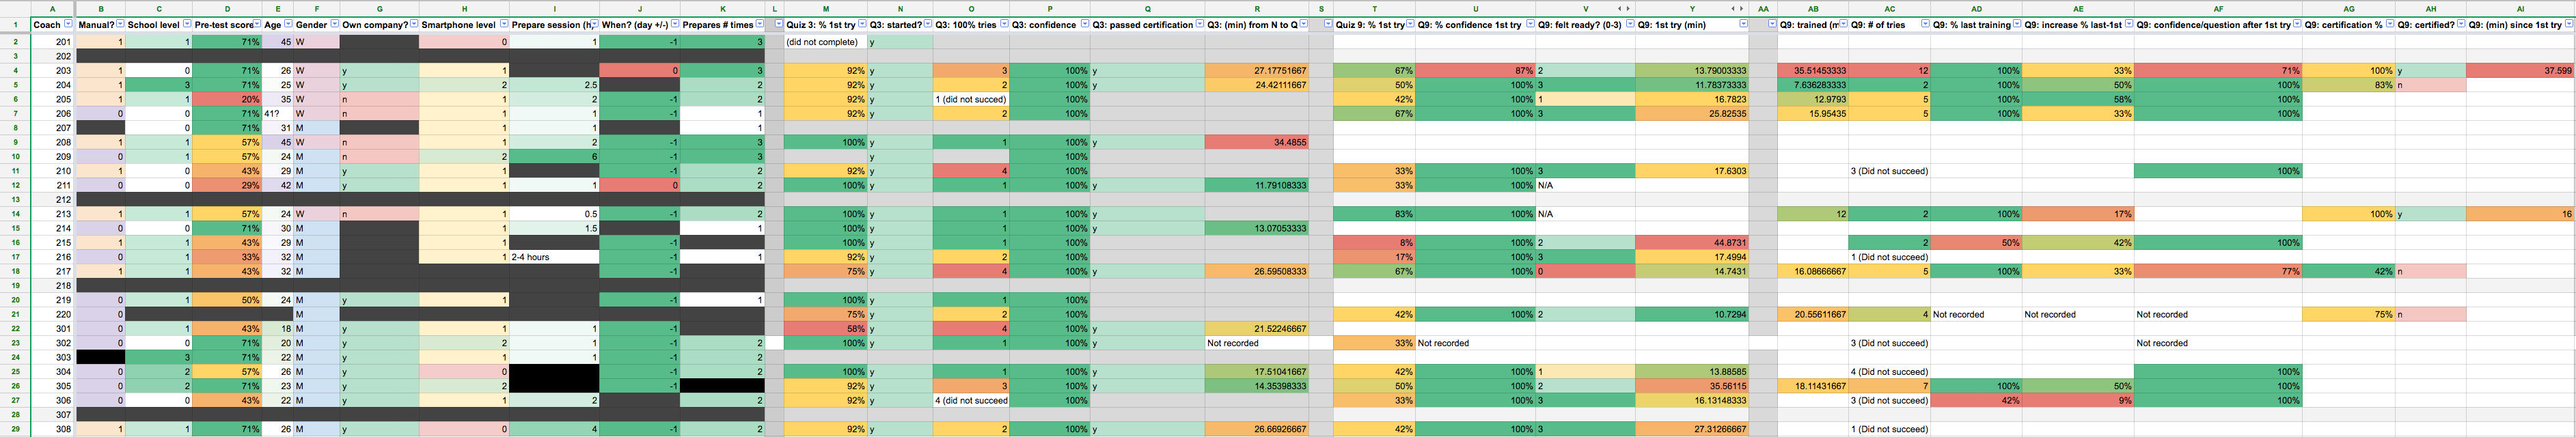
\includegraphics[width=1.0\textwidth]{analysis/sheets/0Overview.png}
    \caption{The multi-variate data set, made filterable and sortable in Google Sheets. Color scales and calculating means makes it easier to compare characteristics of the coach together with pre-test and quiz results. However, it is cumbersome and hard to quickly filter data on multiple parameters.}.
    \label{fig:analysFarg3}
\end{figure}

To meet the challenges of using Google Sheets, a multivariate analyzation software or a visualization was suggested to discover the data in less time. It was hard to determine a suitable multivariate analysis software suitable when having so few data points. Principle Component Analysis or Cohen's kappa would not be suitable, neither was it believed applicable to do Linear correlation on all dimensions. After discussion with other Master thesis students working with analysing data from various disciplines, parallel coordinates was suggested. It would allow very quickly filtering of the data, finding correlations, and distinguish outliers and common characteristics.

To guide the usage of the parallel coordinates (as there is so much to discover in the data set), using R to do Logistic correlation was also done. A disadvantage with this method, is that to be statistically significant, many data points may be needed, and it was now known before-hand if the method would be useful. Probably, parallel coordinates would be the best method to analyse a small multi-variate data set.

\subsubsection{Step 6: Visualization Mapping}
The goal with visualization mapping is to generate renderable data, in this case for the parallel coordinates visualization. Thus, a new spreadsheet is added, specific for visualizing the data. Columns were deleted that would serve no visual purpose (for example timestamps), gave all cells data values (even N/A when undefined), deleting users that did not have data, and shortened the column names so they would fit on the screen. The data was then exported from the Google Sheet into CSV.

\subsubsection{Step 7: Rendering}

For rendering, the JavaScript library D3.js, \citep{d3} was chosen. It supports data-driven documents for visualizing data with HTML, SVG and CSS. It supports both JSON and CSV data. A visual framework for multidimensional detectives for D3.js was found called "Parcoords.js", \cite{parcoords}. The example code from "Linking with a Data Table" provided the basis for the rendering. It allowed observing both the parallel coordinates visualization and the table data from the Google Sheet simultaneously.
% https://syntagmatic.github.io/parallel-coordinates/
% Chang, K. (2012). Parallel Coordinates toolkit : Parcoords.js 0.1. Parallel Coordinates toolkit. Retrieved September 8, 2012, from http://syntagmatic.github.com/parallel-coordinates/
% Kosara, R. (2010, May 13). Parallel Coordinates. Eagereyes.org. Retrieved September 8, 2012, from http://eagereyes.org/techniques/parallel-coordinates
% Tricaud, S. (2008). Picviz: finding a needle in a haystack. Proceedings WASL, San Diego. Retrieved from http://www.usenix.org/events/wasl08/tech/full_papers/tricaud/tricaud.pdf

 %https://syntagmatic.github.io/parallel-coordinates/examples/table.html

To work, the example CSV file was replaced with the data from exporting the Google Sheets data. To benefit the visualization, also the colors were changed, and the toolkit's functionality to drag the axes titles around to reorder the dimensions was used, since the goal was to quickly compare and find correlations. The result is visible in \ref{fig:parallell-coordinates-1}.

\begin{figure}[h]
    \centering
    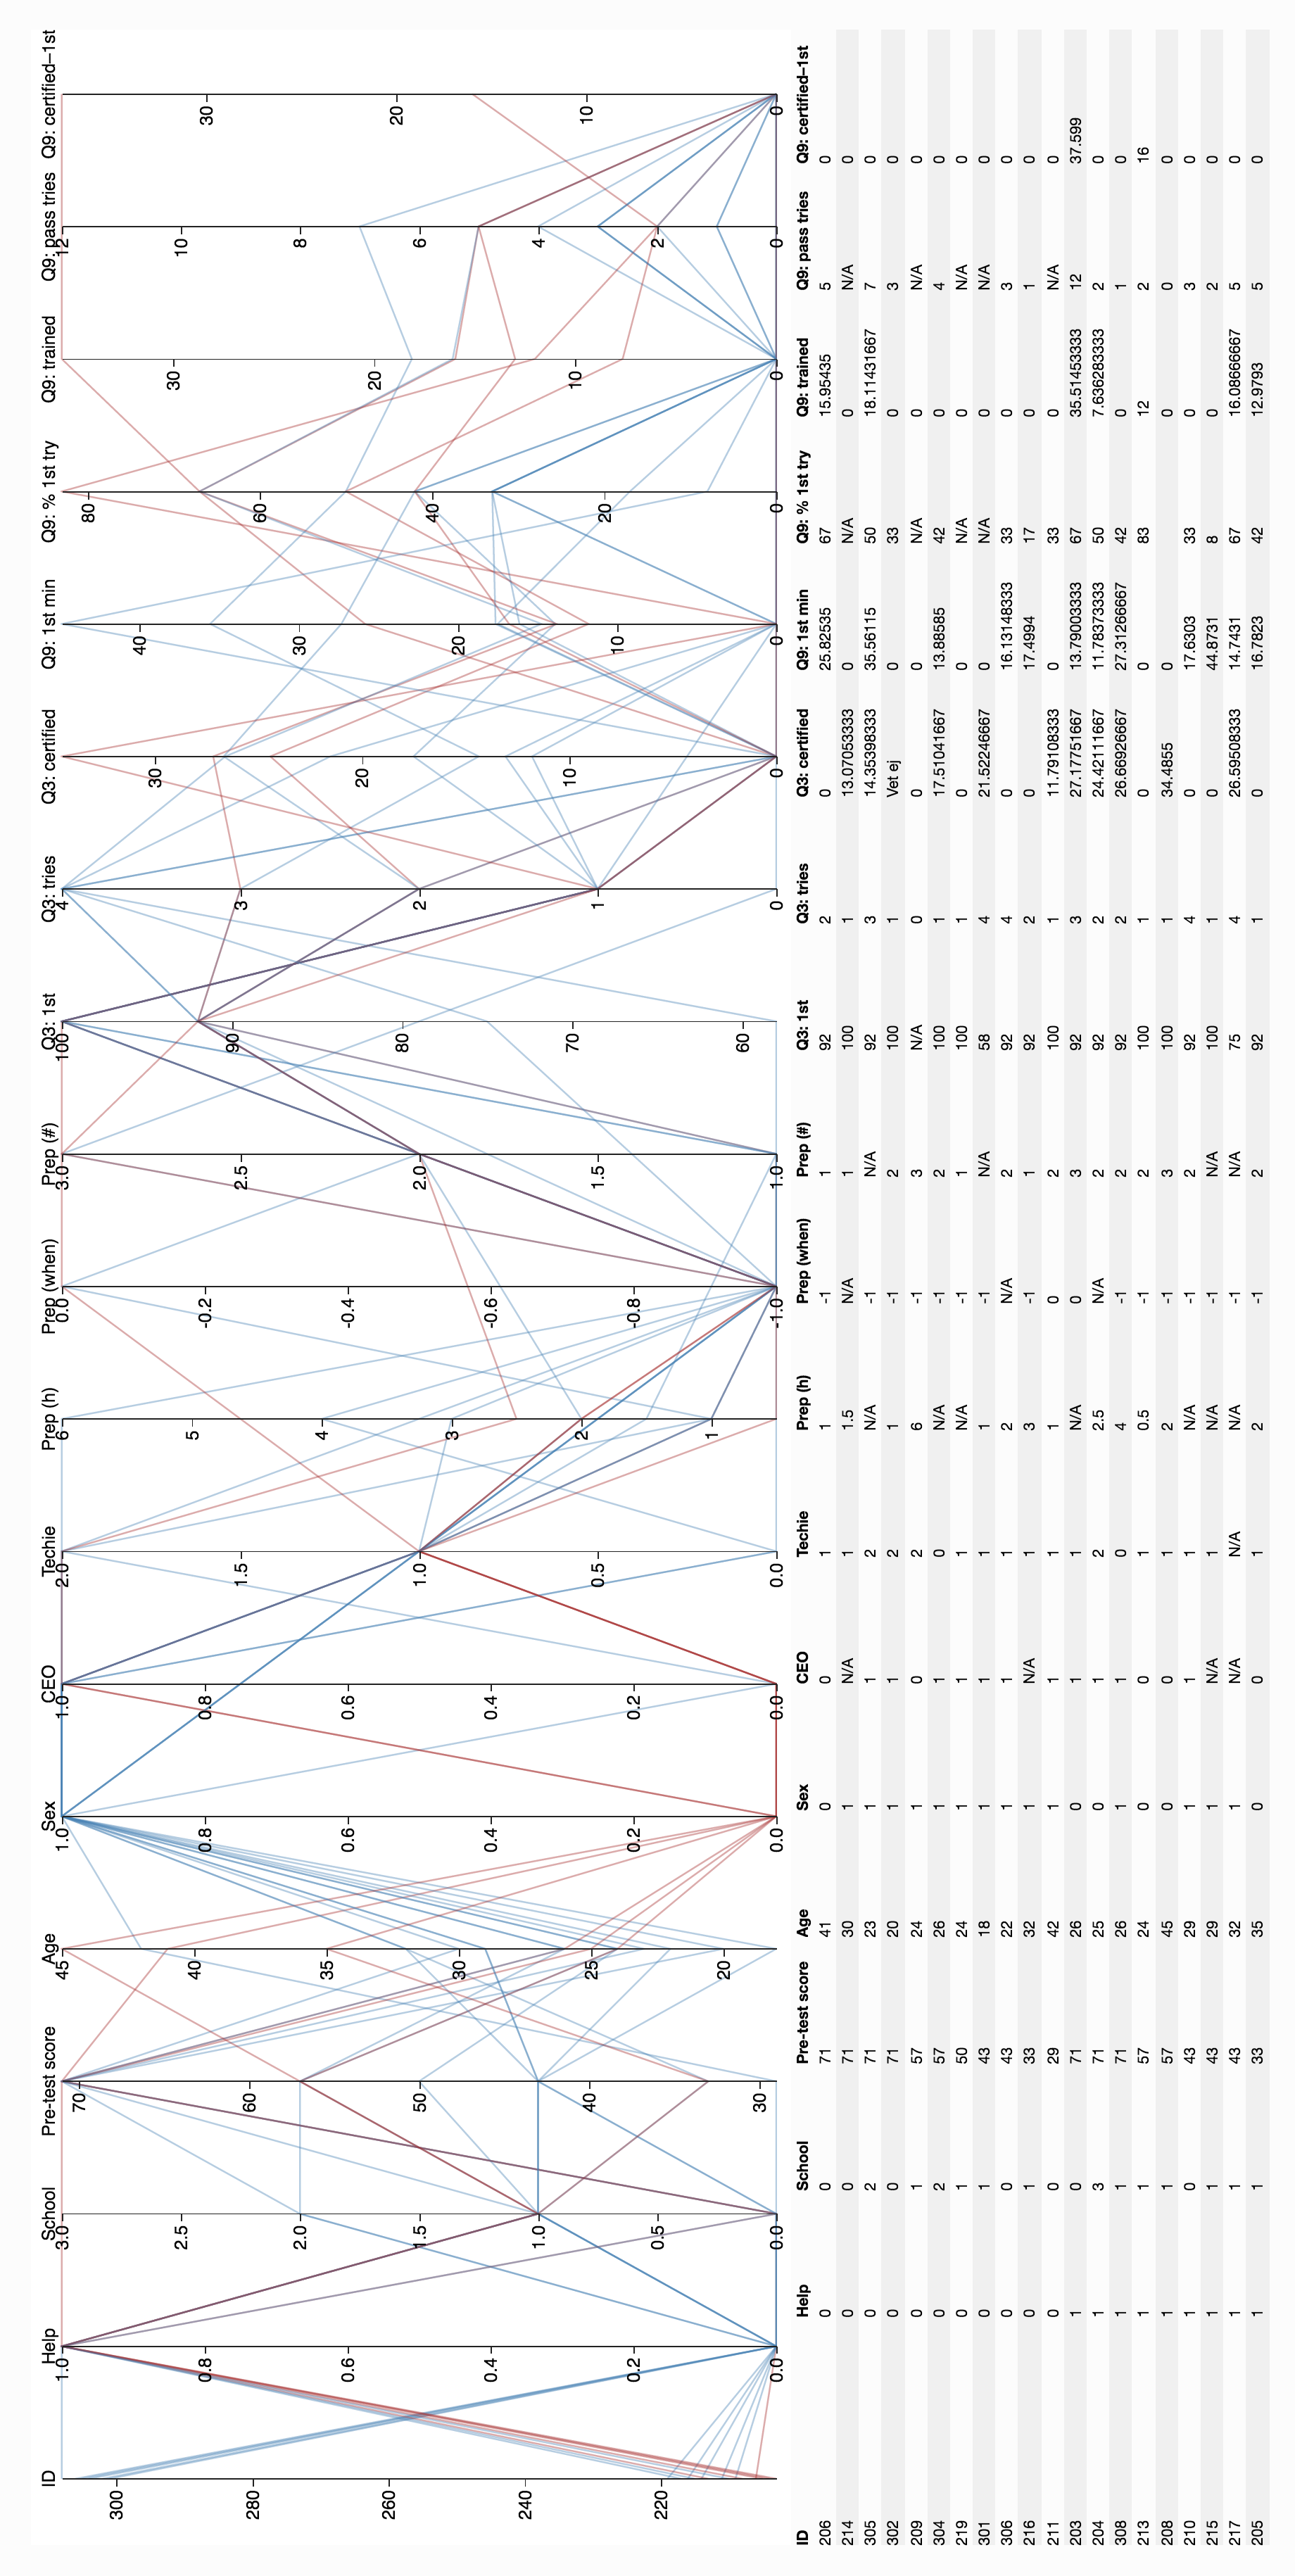
\includegraphics[width=0.7\textwidth]{analysis/parallellCoordinates3.png}
    \caption{The parallel coordinates visualization, done in d3.js. The visualization support draggable axes, filtering of data via dragging the sliders (which synchronizes with the data table), color assignment (like blue and red for men and women in the example), and hovering over a specific data point.}
    \label{fig:parallell-coordinates-1}
\end{figure}



% Application implementation
\section{Application Implementation}

In this section, the prerequisites for the app is described, from the perspective of the user, stakeholders, and the developer.

\subsection{User Needs}

The technical constraints for the project, would need to affect the technologies used, if the project would be user-centered.

On the client side, the app would need to be mobile and web based, consider non-access to internet, and not use a lot of battery, to work for the coaches of YoungDrive.

That the app should be simple to use in this cultural setting leaded to design constraints and needs for evaluation.

\subsection{Stakeholder Meeds}

As the project was only three months, and the first month would be without digital development, time constraints were massive. However, to be able to answer research question \#2, evaluation needed to be done via data collection.

If no evaluation, there would be no need to write code, instead working with a lo-fi prototype using pure design tools. Now, a data-driven approach was needed to measure, and therefore an app needed to be developed.

On the server side, a database and API would be needed, to pull data from the database and push data from the client. Since internet was not always available, the client must be smart in its usage of pushing and pulling data. This would need to be investigated further into the project.

\subsection{Devices to be Used}
As most of the coaches did not have smartphones or tablets, four smartphones (3 Android, 1 iOS) and ten tablets (3 Android, 7 iOS) were brought from Sweden. All of these devices had a web browser and access to an app store. These were either donated, borrowed or bought devices. During the user tests, also using a laptop would be tested.

%\subsection{App/Web Development}
%Early in the project, it was thought that existing tools could be used, instead of building the app from scratch. E.g. using existing tools like Knowly or Typeform\footnote{examples include https://showroom.typeform.com/to/ggBJPd and https://showroom.typeform.com/report/njdbt5/dIzi} during the first iterations for understanding users, and during development e.g. the Typeform API (http://typeform.io/). The Typeform API allows developers to create surveys from within their own applications or systems.

\subsection{Choosing Frameworks for Creating the App}

A JavaScript framework helps and speeds up the creation of building web apps. In the start of the project, Meteor \citep{meteor} and Ionic Framework \citep{ionic} were both tested and compared with each other. It was decided that Meteor was the best way forward, partly because it would allow the app to be accessible on the web as well. %\todo{Add from mindmap}

React \citep{react} (a JavaScript library for building user interfaces) was chosen as the front-end framework, having integration with Meteor and being relatively easy to learn and fast for development.


\subsection{Iteration \#2}
Here, the work and result from iteration \#2 is presented.

\subsubsection{Staging environment using Heroku}
Needed when the Meteor free tier was removed. Connected to deploy from GitHub branches automatically. Could have benefitted from CI, passing tests before ready for production. Solved this by having a stage environment (since April 19th) where stage is YoungDrive-beta (branch Iteration 4), and YoungDrive is master.



For iteration 3, as components grew, there was a need for a client-side router. The Meteor plugin Flow Router was used, as it was very popular with good integrations.

For iteration 3, there was also a need to store data per individual, partly because the feature was prioritized from YoungDrive, but also because of the purpose of data collection. In order to store data per individual, a database and login would be needed. Because of technical difficulties, login and automatic data collection was not implemented until iteration 4, which can be read more about in the Discussion in \ref{backwards-capability}.

\subsection{Login}
To record data per user, would require login. This would be a usability issue for most problems, being 1st-time smartphone users. They need to find it intuitive, user-friendly, and be able to remember the password in the future. A lot of different suggestions were through the ideation phase.

The simplest login possible was chosen, after evaluation and discussion with experts: a 3-digit code, which was to be given to each coach during the test.

%Jag pratade med flera om detta, Expedition Mondial och Grameen. Från EM lärde jag mig att de trodde min idé med en färdiggjort lista med coachernas namn (vi vet ju vilka som är i Tororo) skulle fungera, och från Grameen fick jag höra om dera erfarenhet att de validerat använda samma approach, med en PIN (längre än 4 siffror dock), men att de inte nailat konceptet ännu, och att de också itererar på sin approach för nästa uppdatering av LedgerLink.

Meteor had limitations with their auto-login module, which is very fast to implement. It forces username and password, and instead I wrote the login myself. This was

To summarize, the front-end was not problematic, however, implementing server-client communication so that it worked online and offline, was.

%Tyvärr har också Meteor begränsningar med deras auto-login-modul. Den tvingar både användarnamn och lösenord, och har automatiskt registrering. Går det att stänga av? Jag kan skapa användare och lösenord åt alla, och funderade på hur jag skulle generera lösenord. Ett förslag blev att bara registrera deras förnamn, och sedan skapa lösenordet baserat på T9 med de 6 första bokstäverna utan att berätta det för dem. Sedan tänkte jag på det kulturella, att det kan vara oartigt med förnamn, och bestämde mig för efternamn istället. Hela namnet skulle bli för långt och krångligt.

%Helst skulle jag behöva gå runt Meteors standard-inloggning, och istället ha en enkel login-rullista som den ovan beskrivet, istället för att använda deras standard-lösning.

\subsubsection{Online and offline database}
If data was to be sent from the client to the server, there needs to be a database with Meteor Collections. An example app was made first, only using Meteor Collections. Meteor's use of Distributed Data Protocol (DDP), made app pushes feel immediate, even though data was not sent until there was Internet access.

However, it was found out that if it took more than 15 minutes to get online, the push would be aborted. For users that are seldom online, this would not be viable.

An offline database was needed, and the plugin GroundDB was implemented. As it was cumbersome to get right, pushing the data whenever online, and hard to test (needed to wait 15 minutes each time), this was not ready for the interactions until Iteration 4. As a consequence, until iteration 4 of the app, no results were saved online via the app whatsoever.



For iteration \#4, data collection was done by the app itself, which pushes data to server whenever online (it saves quiz start, and quiz finish). The server receives JSON data from the client, stored in the MongoDB database hosted on Heroku. Each data point is saved in a database called Results, with the signed in user (from the Users database). In the database, there are collections for Users, Quiz Lists, and Quiz Results.



